\documentclass[12t, letterpaper]{article}
%, titlepage
\usepackage[left=1in, right=1in]{geometry}                % See geometry.pdf to learn the layout options. There are lots.
%\geometry{letterpaper}                   % ... or a4paper or a5paper or ...
%\geometry{landscape}                % Activate for for rotated page geometry
%\usepackage[parfill]{parskip}    % Activate to begin paragraphs with an empty line rather than an indent
\usepackage{graphicx, subfigure}
\usepackage{amssymb}
\usepackage{epstopdf}
\usepackage{amsmath}
\usepackage{setspace}
\usepackage{amsthm}
\usepackage{natbib}
\usepackage{booktabs}
\usepackage{rotating}
\usepackage{multirow}
\usepackage{pbox}
\usepackage{url}
\newtheorem{hyp}{Hypothesis} 
\usepackage{appendix}
% \usepackage[nolists, nomarkers, heads]{endfloat}
\setcounter{secnumdepth}{2}
\usepackage[T1]{fontenc}
%\usepackage{fourier}

\def\citepos#1{\citeauthor{#1}'s (\citeyear{#1})} % possessive citations


\DeclareGraphicsRule{.tif}{png}{.png}{`convert #1 `dirname #1`/`basename #1 .tif`.png}


\author{Andrew W. Pierce \\ University of Georgia \and Steven W. Webster \\ Indiana University-Bloomington}
\title{How Race Influences the Impact of Anger on Trust in Government}
\date{\today}

%\usepackage{Sweave}
\begin{document}
%\Sconcordance{concordance:anger_trust_manuscript.tex:anger_trust_manuscript.Rnw:%
1 7 1 1 0 8 1}


\begin{titlepage}
\maketitle

\thispagestyle{empty}

\begin{singlespacing}
\abstract{whatever}
\end{singlespacing}

\end{titlepage}

%%%%%%%%%%
% end title page %
%%%%%%%%%%

\newpage
\setcounter{page}{1}

\doublespacing

\section{How do Anger and Racial Identity Affect Trust in Government?}
\label{sec:litreview}

\subsection{How Anger Impacts Trust In Government}
\label{subsec:angertrust}

Many factors have been found to shape trust in government. Perhaps the most notable -- and most studied -- factor that explains variation in citizens' trust in government is one's partisan identity. As \citet{citrin1974} shows, Americans exhibit higher levels of trust in government when their preferred party has control over the governing process in Washington. Conversely, when the opposing party gains power, citizens' trust in government plummets. With the rise of ideological and affective polarization at both the elite \citep{hetherington2001, fap2005} and mass \citep{abramowitz2010, bafumi_shapiro2009} level, the relationship between partisan identity and trust in government has only been strengthened over time \citep{hetherington_rudolph2015}.

Though partisanship is a consistently strong predictor of levels of trust in government, recent work indicates that emotional reactions can powerfully shape an individual's degree of trust in the national government. Indeed, \citet{webster2017} uses an experimental design to show that anger causes individuals to exhibit lower levels of governmental trust. Notably, anger's ability to lower trust in government does not depend upon the specific target of the anger. On the contrary, both political and apolitical anger have been found to attenuate citizens' trust in their own government.

This finding, and others like it that study the role of emotions in politics, is largely rooted in the findings of Affective Intelligence Theory \citep{marcus_etal2000}. Rather than conceptualizing emotion and reason as separate domains that independently influence an individual's approach to (and evaluation of) the political world, Affective Intelligence argues that emotion and reason are interconnected processes. In fact, emotion and reason are so intertwined that emotions oftentimes influence both what people think about and how they think about these things. The specific ways in which emotions affect cognition and public opinion are varied, though emotions that have a negative valence (such as anger, anxiety, or fear) tend to cause people to render poor assessments of the object being evaluated. On the contrary, emotions that have a positive valence (such as happiness or optimism) often lead individuals to give positive evaluations of people, places, or institutions \citep{bower1991}.

Notably, anger is an emotion that contains a negative valence. Thus, individuals who are made to be angry will tend to evaluate people or objects in a negative fashion. Such anger-induced poor evaluations have been found to affect phenomena as diverse as artwork \citep{silvia2009looking}, companies \citep{bennett1997anger}, and information about crises \citep{kim2011emotions}. Accordingly, we should expect the relationship between anger and trust in government to operate similarly. Higher levels of anger should lead to lower evaluations of the national government, expressed via the pathway of lower levels of trust.

\subsection{How Racial Identity Impacts Trust in Government}
\label{subsec:racetrust}

Understanding how race impacts trust in government can be understood in the various ways trust in government is defined, and the degree to which that definition is shaped by an individual's racial identity. Early definitions of trust in government considered two possible ways in citizens could evaluate their governments: the degree to which they trusted in the political system and degree to which they trusted the political regime \citep{easton1965}. This is to say that citizens can ``trust'' the government in a least two different ways. In the first way, individuals evaluate the likelihood of government systems and institutions to treat them fairly. In the second meaning, individuals evaluate the likelihood of the individuals and parties in charge of the government to treat them fairly. 

Contemporary work has explored the degree to which partisanship influences trust according to the second definition. Given the degree to which parties pursue different policies in office, it follows that partisans would evaluate the likelihood of the current government to treat them well on the basis of which party was in charge.  \citet{keele2005} finds that, in the context of American politics, an individual's trust in government depends to a large degree on the party of the individual and the party in charge; generally, partisans trust the government less when the opposition party is in charge. Furthermore, he finds that this pattern is consistent since the 1950s, and that independents are much less likely exhibit strong swings in trust based on the party in charge. These findings are corroborated by \citet{cook2005}, who find that the type of trust measured in national surveys like the ANES tend to measure an individual's trust in the current regime as opposed to the overall political system. 

While partisanship is an important predictor of trust when considering a current political regime, racial identity has been shown impact how individuals are evaluating government. \citet{wilkes2015} notes that, given the long history of institutional discrimination faced by black Americans due to their racial identities, black Americans likely evaluate the fairness and trustworthiness of the government in different ways than white Americans. Using data from the ANES covering years from 1985-2012, \citeauthor{wilkes2015} finds that black Americans exhibit patterns of trust that would support both a regime-oriented and system-oriented framework for evaluating the American government. Contrary to what one might expect given the history of racial and ethnic tensions in the US, both black Americans and Latinos appear to have higher levels of political trust than white Americans\footnote{See \citet{wilkes2018} for a broader review.}.

Why might levels of trust vary by race? \citet{nunnally2012} argues that the specific political socialization of black identity means that black Americans process and express trust in different ways than white Americans. Specifically, black Americans have received a unique socio-cultural message, i.e. socialization, about what it means to be black in America as well as the level of trust that can be afforded to other groups. This message, which is shaped by years of legal discrimination and exclusionary politics by different parties at different times, directly impacts the degree to which black Americans will trust a person or party in contrast to the broader system of government.\footnote{This is not to say that all black Americans receive the same racial socialization message or that levels of trust in government among black Americans is monolithic. Rather, as \citeauthor{nunnally2012} shows, there is substantial heterogeneity in levels of trust among black Americans.}. From this perspective, it makes sense to expect that the psychological processing and evaluation of trustworthiness of the government varies significantly between racial groups.

Beyond a white/black dichotomy, other ethnic groups in the United States display differing levels of trust based on differing socialization as well. For immigrant groups who experience political socialization through acculturation, may be incorporated into the American political system and its norms based on differences in legal status and time of stay in the United States \citep{uslaner2003}. Interestingly, several scholars have found that higher levels of acculturation lead to \textit{decreased} trust in government among immigrant groups \citep{abrajano2010,michelson2001}. This is in contrast to the generic aggregate (white) experience, where trust and engagement tend to support each other \citep{uslaner2005}. 

\section{How Race Modifies the Influence of Anger on Trust}
\label{sec:theory}

%\subsection{Pierce Edits}

How, then, does racial/ethnic identity impact the influence of anger on trust in government? Although both groups express trust in government at the regime and system political levels, Whites and non-Whites experience political systems in different ways as a function of different socialization experiences\footnote{See also the work of \citet{humphries2013} who show how similar socialization experiences of white children and immigrant children lead to different levels of participation as adults.}. Because socialization experiences differ between whites and non-white, we also expect anger -- and especially political anger -- to be processed differently between Whites and non-Whites. In other words, if the way in which Whites and non-Whites relate to the political system and its actors differ significantly, as prior research has shown, then we expect the evaluation of government through the lens of anger to differ as well.

Such an expectation has considerable grounding in the existing literature. \citet{phoenix2019}, for instance, has shown that Black and White Americans express different amounts of anger about politics. While White Americans frequently express anger, Black Americans tend to be more reserved in their expression of this emotion. This racial difference has produced an ``anger gap" -- a gap that leads to different mobilization actions according to one's racial identification. Related work has found similar differences in anger's ability to shape political behavior and public opinion across race. Indeed, studies have shown that anger activates racial resentment among White Americans \citep{banks2014} and causes Black Americans to donate to political groups that are specifically focused on advancing the interests of Black Americans \citep{banks_white_mckenzie2019}.

Differences between the socialization and political incorporation of Whites and non-Whites, as well as the documented racial differences in the political implications of felt emotions, suggest two possible theories how governments are evaluated in the presence of anger. The first theory, which we will call system anger, holds that anger shapes trust by connecting negative emotion to broader beliefs about the political system. 

The second theory, which we will call specific anger, holds that anger shapes trust by connecting negative emotion to a particular party or regime. This theory, much like theories of negative partisanship\footnote{See e.g. \cite{abramowitz2016}} suggests that negative feelings greatly shapes a person's beliefs and behaviors. If, as is likely the case in American politics, parties broadly fall along racial and ethnic cleavages, then negative affect may be processed through partisan lenses as well. Thus, nonwhites, for whom racial/ethnic politics are a dominant political topic, will process negative emotions through negative trust in regimes.

We hypothesize two particular avenues by which anger might impact trust in different ways between whites and non-whites. On the one hand, it may be the case that anger provokes negative emotion with respect to system trust. If this is the case, then we would predict that whites would show a stronger relationship between anger and trust nonwhites because of the more persistent diffuse support among non-whites. However, if anger affects specific trust for political regimes, then we would suspect that nonwhites would exhibit a stronger relationship between anger and trust as the fortunes of non-whites are much more tied to specific partisan regimes.

%\subsection{Webster Edits}

%By combining earlier research that anger decreases trust in government and that trust is granted by different racial groups in different ways, we theorize that nonwhite Americans filter trust through anger in a different way than white Americans. Specifically, we hypothesize that nonwhite Americans will express greater levels of distrust than white Americans when experiencing similar levels of anger. Such an expectation is rooted in recent work that has suggested that White and non-White Americans interact with the political system in different ways.

%\citet{phoenix2019}, for instance, has shown that Black and White Americans express different amounts of anger about politics. While White Americans frequently express anger, Black Americans tend to be more reserved in their expression of this emotion. This racial difference has produced an ``anger gap" -- a gap that leads to different mobilization actions according to one's racial identification. Related work has found similar differences in anger's ability to shape political behavior and public opinion across race. Indeed, studies have shown that anger activates racial resentment among White Americans \citep{banks2014} and causes Black Americans to donate to political groups that are specifically focused on advancing the interests of Black Americans \citep{banks_white_mckenzie2019}.


\section{How does the impact of anger on trust compare between whites and non-whites?}
\label{sec:design}

Our empirical investigation of the ways in which race might be shaping the impact of anger on trust in government will proceed in three parts. First, we will offer a replication of analysis presented by \citet{webster2017}, but extend that analysis to the 2016 American National Elections Study and the 2012 Outlook on Life Survey. Second, we will present analysis using a  Bayesian Additive Regression Tree (BART) model which allows us to explore the possibility of hetergenous effects suggested by our initial analysis. Finally, we will offer results of a survey experiment confirming our observational analysis.

\subsection{Extending Prior Analysis}
\label{subsec:anes}

To examine how racial identity conditions the relationship between anger and trust in government, we first begin by utilizing data from the 2016 American National Election Studies (ANES). The ANES is useful for our purposes because, in addition to its large sample size, it contains the three variables essential to this analysis: a measure of trust in government, measures of anger, and information about each respondent's racial identity.

Though there are many possible ways to measure trust in government, here we are focused on one specific aspect of governmental trust: respondents' perceptions of whether public officials care about what people think. This measure is captured by asking individuals to rate their level of agreement with the following statement: ``public officials don't care what people think." Responses take on five possible values, ranging from ``disagree strongly" to ``agree strongly." We then recode this variable numerically to range from 0-4, where higher values indicate higher levels of \emph{dis}trust in government.

To measure individuals' level of anger, we analyze the frequency with which individuals reported feeling angry at the opposing party's presidential candidate. Thus, for Republican respondents, our measure of anger captures how often he or she felt angry toward Hillary Clinton. Similarly, for Democratic respondents, our measure of anger captures how often he or she felt angry toward Donald Trump. We normalize this variable to range from 0-1, where zero indicates that an individual never felt angry toward the opposing party's candidate and one indicates that an individual reported that they ``always" felt angry toward the opposing party's candidate. 

Finally, to analyze how an individual's racial identity conditions the relationship between anger and his or her level of trust in government, we utilize individuals' responses to the question asking about racial affiliation. Potential responses are White, non-Hispanic; Black, non-Hispanic; Asian, native Hawaiian or other Pacific Islander; Native American; and Hispanic. We then collapse responses to this question into a dummy variable indicating whether an individual identifies as something other than White. Though this obscures any potential differences in the ways in which specific non-White racial identities condition the relationship between anger and trust in government, this approach allows us to establish a baseline as to whether such racial differences exist at all.

At the highest level, we find that anger has a positive and significant impact on trust in government. Increasing levels of anger are associated with lower levels of trust in government at statistically significant levels and on an order of magnitude similar to that found prior analysis of the 2012 ANES \citep{webster2017}.\footnote{A full model replication between the 2012 ANES and 2016 ANES can be found in the appendix, the results from 2016 replicate the results in 2012 in direction and magnitude} Because results from earlier analyses generalized across races, we include an additional interaction term between the white/non-white dummy variable and the ordinal anger variable, which will allows to compare the effect of anger between whites and non-whites.

Previous research has shown interaction effects to best be understood through visual interpretation, as proper analysis requires evaluating the interaction at all values of interest \citep{brambor2006}. Accordingly, we present a graphical analysis of the interaction effect showing the effect of anger on trust in government conditional on racial identity.

To estimate whether racial identity conditions the relationship between anger and trust in government, we employ a series of Bayesian Additive Regression Tree (BART) models. Unlike traditional linear models, BART models do not impose any linearity conditions on the data. Moreover, BART models produce an estimate as to the relationship between anger and trust in government for each individual in our data. Thus, we are able to easily examine potential non-linearities between anger and trust in government, as well as the ways in which racial identities condition this relationship. To reduce confounding in our estimation we also include controls for individuals' self-reported ideology, their gender, their level of education, their degree of political activism, and pre-election levels of trust in government.\footnote{The political activism scale is an additive measure of 11 different campaign-related activities. These activities include attending political meetings; talking to others about politics; wearing a campaign button; working for a political party; contributing money to a party, candidate, or third-party organization; joining a political protest; attending a school board meeting; contacting a Member of Congress; and signing a petition.} The results of the BART model are shown in Figure \ref{fig:bart-results}.

\begin{center}
\begin{figure}
\begin{center}
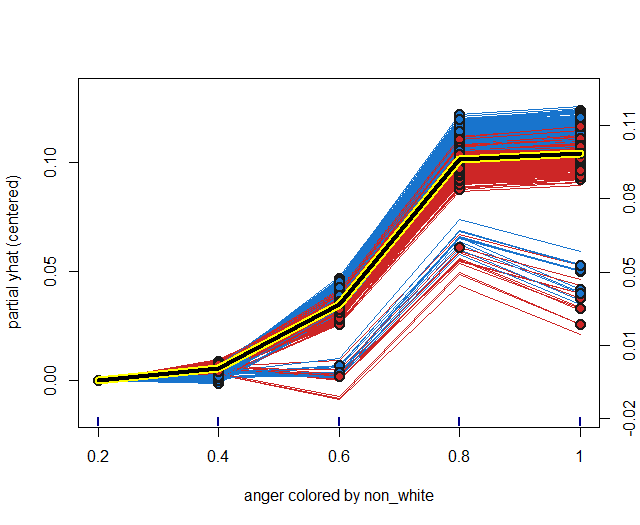
\includegraphics[width=\textwidth]{bart_model}
\caption{\footnotesize\textit{Anger, Race, and Trust in Government.} This figure shows the non-linear relationship between anger and trust in government. It also shows that the relationship between anger and trust in government is stronger for those individuals who identify as non-White.}
\label{fig:bart-results}
\end{center}
\end{figure}
\end{center}

The results of the BART model displayed in Figure \ref{fig:bart-results} reveal two interesting patterns. The first is that the relationship between anger and trust in government is non-linear. As can be seen, there is very little relationship between anger and trust in government at low levels of individual anger. When individuals move into the middle range of anger there appears to be a slightly more detectable relationship between anger and trust in government. However, when individuals exhibit the highest levels of anger there is a strong connection between anger and distrust in the national government. Indeed, the jump from the median level to the next highest level of anger produces a dramatic increase in the likelihood that an individual distrust the government. This relationship increases slightly more when individuals are at the highest level of anger. Accordingly, these patterns suggest that, though anger is certainly related to distrust in government, this distrust is most readily manifested when individuals are exhibiting high levels of anger.

The second pattern that emerges from the BART model displayed in Figure \ref{fig:bart-results} is that the relationship between anger and trust in government is conditioned by an individual's racial affiliation. In Figure \ref{fig:bart-results}, the relationship between anger and trust in government is shaded in red for Whites and shaded in blue for non-Whites. As can be seen, the relationship between anger and trust in government is stronger for non-Whites at almost every level of anger. Indeed, it is only at the very lowest levels of anger that the relationship between anger and trust in government is stronger for Whites than non-Whites. At every other level of anger, the results of the BART model suggest that anger is more closely related to distrust in government for non-Whites than for Whites.

\subsection{Experimental Design}
\label{subsec:experiment}

The preceding analysis has established that anger is related to trust in government, that this relationship is non-linear, and that the relationship between these two variables is stronger for those who are non-White than for those who are White. However, as the model presented in Figure \ref{fig:bart-results} relies on observational data, it is not possible for us to say from these results that anger causes distrust in government, nor does it allow us to say that the causal effect of anger on governmental distrust is stronger for non-Whites than for Whites.

To explore whether the relationship between anger and trust in government is causal in nature, we employ a survey experiment that exogenously varies individuals' level of anger. The survey experiment was fielded throughout the country in the fall of 2016 via Survey Sampling International (SSI) and was finished a few months before the U.S. presidential election. The experimental data is comprised of 3,262 respondents, all of whom are registered to vote in the United States. 

The data for this study contains a pre- and post-experiment survey. Before the experiment, participants were asked to fill out a series of demographic questions. These questions include the respondent's year of birth, gender, race, yearly income, and and level of education. Participants were also asked a series of political identification questions. These questions include an individual's partisan affiliation and ideological leanings, both of which are measured on a seven-point scale.\footnote{These questions are analogous to those used in typical datasets, such as the American National Election Studies or the Cooperative Congressional Election Study.} Individuals were also asked about their past forms of political participation and level of interest in politics and political affairs.

The experimental manipulation of the study is designed to increase individuals' level of anger. In order to do this, we rely on a technique known as ``emotional recall" \citep{lerneretal2003effects, lerner_kelter2001}. This manipulation asks individuals to write a detailed paragraph about a time they felt a given emotion (here, anger), with the expectation that writing about their experience will cause an individual to temporarily relive the triggered emotion. Such a design has become widespread in political science, and has been most notably used to study the effect of emotions on Americans' views toward terrorism \citep{lerneretal2003effects}, likelihood of participating in politics \citep{vbggh}, and seeking information about politics \citep{valentinoetal2008}.

However, the experimental manipulation used in this study differs from previous uses of the technique in an important way. Typical emotional recall designs ask individuals to recount a time that they felt a particular emotion about politics. By phrasing the experimental prompt in such a way, it is likely that scholars are unintentionally introducing confounding considerations into their designs. Indeed, when the experimental prompt is phrased in such a way, it is impossible to tell whether individuals are reacting to a prompt to exhibit a higher degree of some emotion, or if they are responding to the increased salience of politics or political issues. In order to disentangle this methodological problem and obtain more valid estimates as to the causal effect of anger on rational miscalculations, the experimental recall design that we use separates the emotion (anger) from the target (politics) \citep[see also,][]{webster2017}. Thus, our design randomizes individuals into one of three treatment groups. In the first treatment group, individuals are asked to recall a time they were very angry, and to describe this time in such a way that an individual who was reading the response might also become angry. The second treatment group asks individuals to write about a time they were very angry specifically about politics, while the third treatment group asks individuals to write about a time they thought about politics. This simple modification of the experimental wording allows us to avoid concerns about confounding factors that plague other studies and, as a result, be more certain that the experimental manipulation is altering levels of anger and \emph{not} merely increasing the salience of political issues.

After the experimental manipulation, subjects were asked to rate their level of agreement or disagreement with the following statement: ``The national government is unresponsive to the concerns and interests of the public." Agreement is assessed on a 0-10 scale, where higher scores indicate more agreement. Thus, higher values indicate a greater level of distrust in the national government.

The unconditional expectation is that those individuals who were randomized into one of the two anger-inducing treatment groups should be more distrustful of the national government. In other words, they should give higher ratings on the post-experiment question about the government's responsiveness to the concerns and interests of the public. However, the key focus of this paper is how the relationship between anger and trust in government is moderated by the race of the respondent. As described in Section \ref{sec:theory}, our expectation is that the effect of anger on reducing trust in government should be stronger for non-Whites. Given the randomized nature of the experimental design, estimation occurs via a simple ordinary least squares (OLS) model as shown in Equation \ref{eq:experiment-model}.

\vspace{-13mm}
\begin{center}
\begin{equation}
y_i = \alpha + \beta_1 Anger_i + \beta_2 PoliticalAnger_i + \beta_3 PoliticalSalience_i + \epsilon
\label{eq:experiment-model}
\end{equation}
\end{center}

To test for heterogeneous treatment effects by individuals' racial affiliation, we subset the model shown in Equation \ref{eq:experiment-model} to include only those individuals who racially identify as something other than White. Estimating our model only on the subset of individuals who identify as non-White functionally achieves the same thing as including a series of dummy variables for non-White respondents and interacting them with the indicators for treatment status. However, to facilitate a comparison of the relationship between anger and trust in government for Whites and non-Whites, we also estimate Equation \ref{eq:experiment-model} on the entire sample. We then simultaneously present the results of these two models in Figure \ref{fig:coef_plot}.

The results of our experimental analyses largely corroborate the results of our observational analysis. Indeed, the results of our experimental manipulation suggest that the strength of the relationship between anger and reduced trust in government is dependent upon one's racial affiliation. Recall that the expectation is that those individuals who were randomized into one of the treatment groups that sought to prime anger should be more distrustful of the national government. Mechanically, this implies that the coefficient on the treatment indicators for the anger-only condition and the anger-about-politics condition should be positive. The results, shown in Figure \ref{fig:coef_plot}, provide a considerable amount of support for this hypothesis.

The results indicate that anger has differential effects depending upon whether an individual is White or non-White. Among White participants ($n=2666$), apolitical anger increases distrust in the national government ($p < .05$) as does targeted political anger ($p < .1$). Merely thinking about politics does not have any statistically significant effect on trust in government. The results for non-White participants ($n=586$) are slightly different. Among non-Whites, apolitical anger has no statistically discernible effect on lowering trust in government. However, non-White individuals who were randomized into the targeted political anger condition exhibit a greater amount of distrust in the national government than White individuals who were randomized into this same treatment condition. Moreover, for non-White experiment participants, merely \emph{thinking} about politics served to reduce trust in the national government. This finding corroborates earlier work by \citet{abrajano2010} showing that higher acculturation and political integration among immigrants leads to lower levels of trust. Taken together, these results suggest that anger's ability to reduce the citizenry's trust in the national government, and the extent to which it does so, is, to a degree, conditional upon an individual's racial identity.

\begin{center}
\begin{figure}
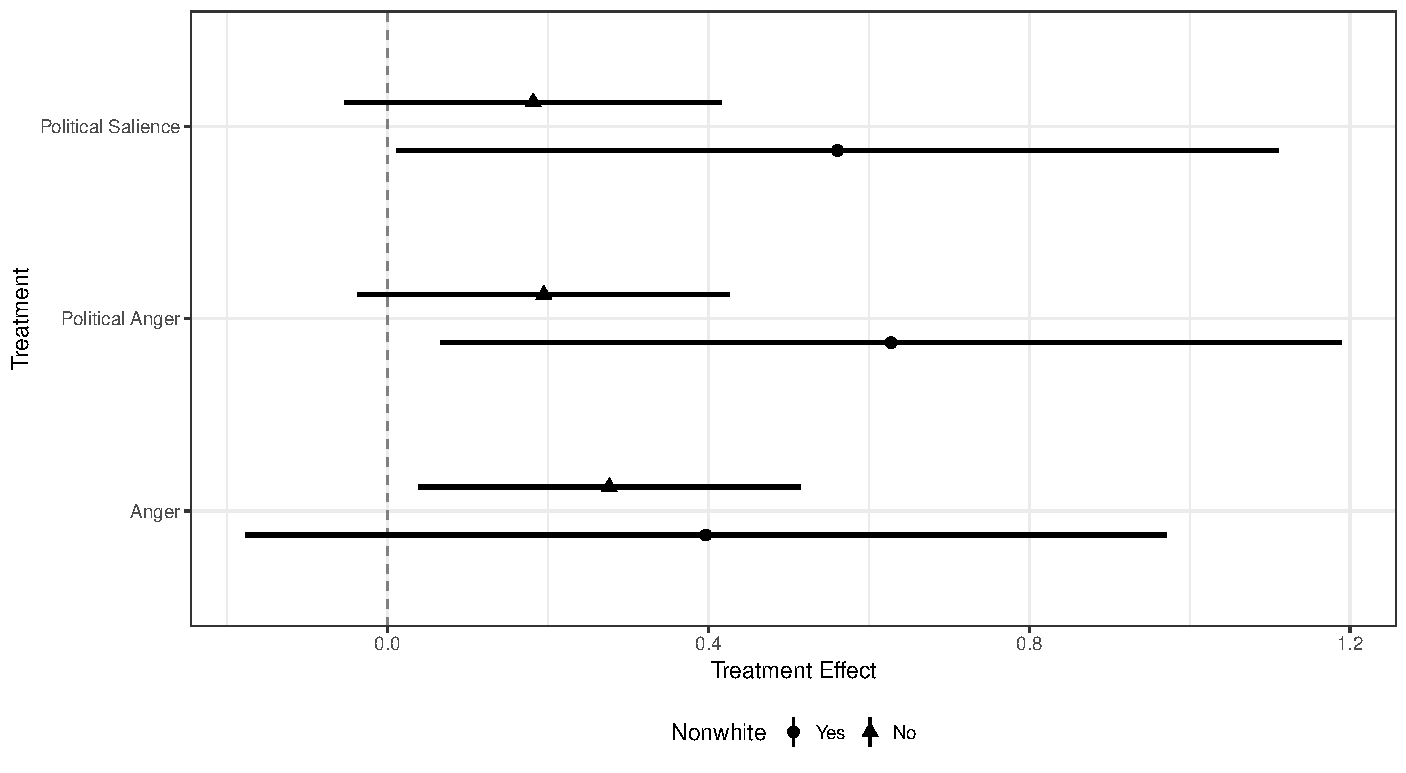
\includegraphics[width=\textwidth]{coefs}
\caption{\footnotesize\textit{The Relationship Between Anger, Race, and Trust in Government.} This figure shows the coefficient estimates from the experimental manipulation that sought to induce anger in participants. The figure suggests that higher levels of anger reduces trust in government and that this effect is greater for non-White individuals.}
\label{fig:coef_plot}
\end{figure}
\end{center}


\newpage
\begin{singlespacing}
\bibliographystyle{apsr}
\bibliography{anger_race_bib}
\end{singlespacing}



\end{document}
